% ========================================================
% --------------------- Evaluation -----------------------
% ========================================================
\section{Evaluation}\label{sec:evaluation}
\setnavsection{sec:evaluation}

\subsection{Effectiveness and Scaling Behavior}
\label{sec:paradigm_effectiveness}

Before giving the downstream-specific results, we first explore whether Orca's core hypotheses hold. As presented in the introduction, Orca is designed to learn a world latent space through next state prediction, and this latent space is expected to support downstream readouts for understanding, prediction, and intervention. Therefore, we evaluate the Orca paradigm by answering two questions:


\begin{enumerate}[label={}, leftmargin=10pt, itemindent=0pt, itemsep=0.3em, topsep=0.3em]
    \item[] \textit{\textbf{$\cdot$ Question 1.1: Is Orca's learning paradigm effective as the model size and data scale up?}}
    \item[] \textit{\textbf{$\cdot$ Question 1.2: Can a stronger latent by pre-training improve downstream readout performance?}}
\end{enumerate}


\subsubsection{Loss of Proposed Learning Paradigm}
\label{sec:evaluation_scaling_loss}

\begin{wrapfigure}{r}{0.38\linewidth}
\vspace{-3.8em}
\centering
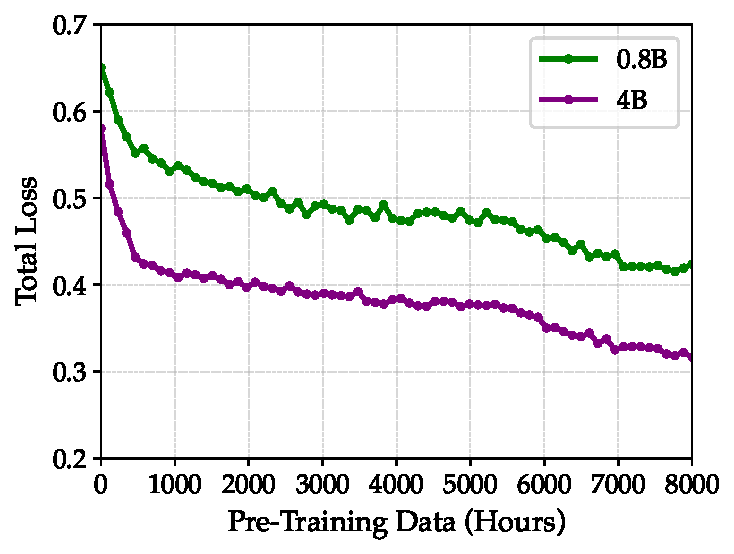
\includegraphics[width=\linewidth]{figs/evaluation/scaling_loss.pdf}
\vspace{-2em}
\caption{\textbf{\small Loss of model and data scaling.}}\label{fig:scalinglaw_loss}
\vspace{-2em}
\end{wrapfigure}


To answer \textbf{\textit{Question 1.1}}, we first performed experiments with model sizes and data scaling, and the loss curves are shown in Figure \ref{fig:scalinglaw_loss}. The horizontal axis represents the amount of pre-trained video data (the unit is hours); the vertical axis represents the total loss, calculated by Equation \ref{eq:total_loss}. The green and the purple lines represent the trends of 0.8B and 4B model sizes, as the data scaling. The total loss has been on a downward trend.



Based on Figure~\ref{fig:scalinglaw_loss}, we obtained \textbf{\textit{Answer 1.1}}:


\begin{enumerate}[label={}, leftmargin=10pt, itemindent=0pt, itemsep=0.3em, topsep=0.3em]
\item[] \textit{\textbf{$\cdot$ Answer 1.1: Orca's learning paradigm is effective and scalable as the model size and data increase.}}
\end{enumerate}

The total loss of Orca decreases as the pre-training data scale up, and the larger Orca achieves a lower objective loss than the smaller one. This trend suggests that Orca provides an \textit{effective} learning paradigm for building world latent. 
Orca does not converge quickly, but rather continuously benefits from more data and larger model sizes. Its loss curve continues to show a significant downward trend, further demonstrating its \textit{scalability}.



\subsubsection{Relationship between latent and downstream readout performance}
\label{sec:evaluation_scaling_performance}

\begin{wrapfigure}{r}{0.7\linewidth}
\vspace{-1.3em}
\centering
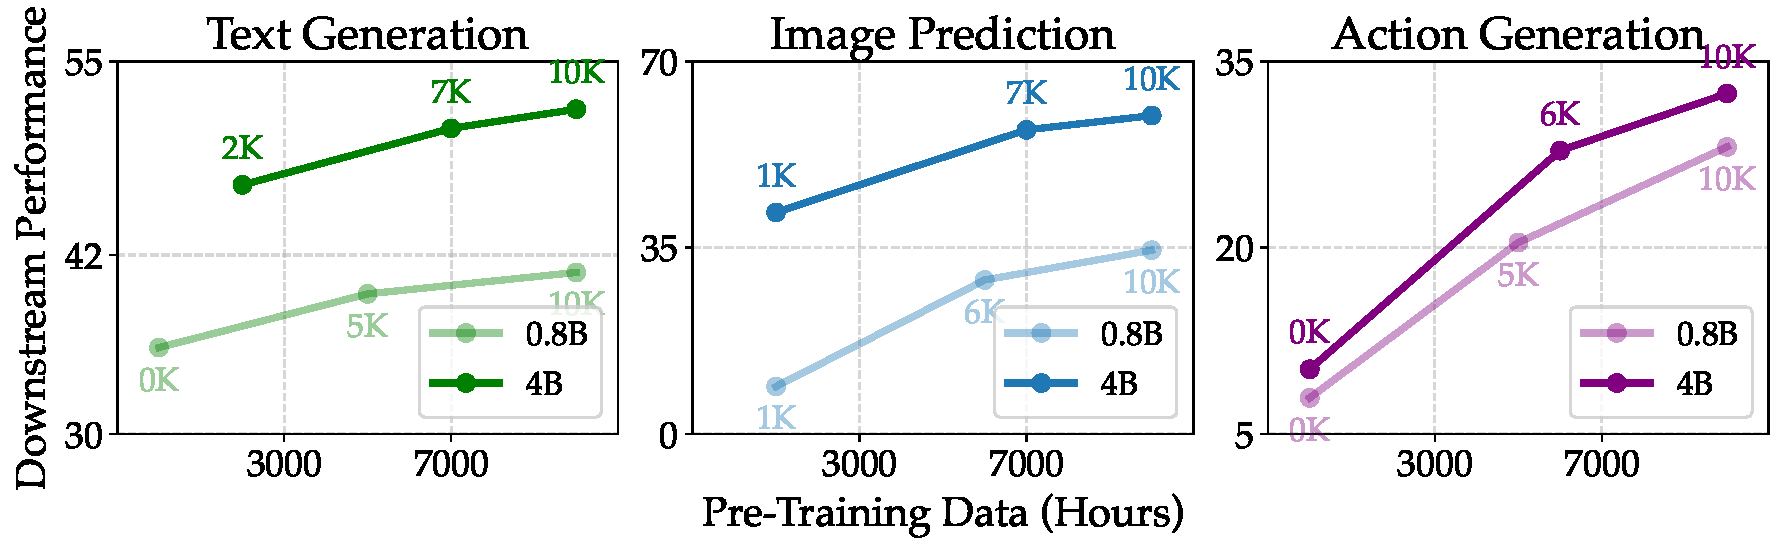
\includegraphics[width=\linewidth]{figs/evaluation/scaling_performance.pdf}
\caption{\textbf{Scaling behavior on downstream readouts performance.}}\label{fig:scalinglaw_readout}
\vspace{-0.5em}
\end{wrapfigure}

To answer \textbf{\textit{Question 1.2}}, we performed probe experiments on Orca-0.8B and Orca-4B. We select some checkpoints from the pre-training process and apply them to downstream tasks to see if a strong world latent can lead to strong downstream readout performance. The readout performance curves are shown in Figure \ref{fig:scalinglaw_readout}.  Light-colored lines represent 0.8B, and dark-colored lines represent 4B. The corresponding points represent probes during pre-training. The horizontal axis is the amount of pre-trained video data, and the vertical axis is the corresponding readout performance.

The downstream readout performance across \textit{text generation}, \textit{image prediction}, and \textit{action generation}. The \textit{text generation} performance is the average performance on four benchmarks: TemporalBench, MVBench, SWITCH, and 3DRSBench. The details are shown in \textbf{Section \ref{sec:evaluation_toL}}. The \textit{image prediction} performance is the average performance of the proposed PRICE-V0.1 benchmark. The details are shown in \textbf{Section \ref{sec:evaluation_toV}}. Note that the above are all zero shots. The \textit{action generation} performance is the average performance on five real-robot out-of-domain tasks. The details are shown in \textbf{Section \ref{sec:evaluation_toA}}.

Based on Figure~\ref{fig:scalinglaw_readout}, we obtained \textbf{\textit{Answer 1.2}}:

\vspace{-1ex}
\begin{enumerate}[label={}, leftmargin=10pt, itemindent=0pt, itemsep=0.3em, topsep=0.3em]
\item[] \textit{\textbf{$\cdot$ Answer 1.2: Stronger world latent from pre-training leads to stronger downstream readouts.}} 
\end{enumerate}

Orca's backbone is frozen during readout post-training. As the pre-training data scale up, text, image, and action readouts all improve. This result shows that Orca's stronger latent space can enhance downstream readout performance. Surprisingly, no data with action labels was used in pre-training, but in \textit{action generation}, this paradigm brought gains by relying on video data. This emergent capability may alleviate, to some extent, the problem of low generalization caused by the scarcity of robot data.


\subsection{Downstream Readout Analysis}

Following the above discussion of \textbf{\textit{Question 1.2}} and \textbf{\textit{Answer 1.2}}, we present the quantitative evaluation results of Orca across three downstream tasks: \textit{text generation}, \textit{image prediction}, and \textit{action generation}. \textbf{\textit{Note that we do not construct or use any benchmark-specific training data for these evaluations, nor do we tune Orca on the evaluation benchmarks.}}



\vspace{-2ex}
\begin{enumerate}
    \item \textbf{\textit{Text Generation}}. It demonstrates the model's out-of-distribution (OOD) commonsense reasoning, comprehension capabilities, and high-level cognitive abilities.
    \item \textbf{\textit{Image Prediction}}. It visualizes this latent cognitive capability through OOD state transitions.
    \item \textit{\textbf{Action Generation}}. It executes the generated actions in real-world OOD scenarios, mapping the state transitions to action manipulation.
\end{enumerate}

\subsubsection{Comparison on Text Generation}\label{sec:evaluation_toL}


To evaluate how state transition modeling enhances abstract reasoning, we conducted text generation assessments on OOD understanding.
The details of benchmarks and baselines of the text generation can be seen in \textbf{Appendix \ref{sec:appendix_evaluation_toL}}.

\paragraph{Benchmarks.} 
We evaluate Orca on a complementary suite of benchmarks that probe different aspects of world-state and state-transition understanding: 
MVBench \citep{MVBench}, TemporalBench \citep{cai2024temporalbench}, 3DSRBench \citep{ma20253dsrbench}, and SWITCH \citep{switch2025}.




\paragraph{Baselines.} We compare Orca with two categories of baselines:

\vspace{-2ex}
\begin{itemize}
    \item \textit{\textbf{World models}}: V-JEPA 2.1~\citep{V-JEPA-2.1}, Emu3~\citep{Emu3}, and Emu3.5~\citep{Emu35}.
    \item \textit{\textbf{Vision-language models}}: Qwen3.5~\citep{qwen35}, Gemma 4~\citep{Gemma4}, DeepSeek-VL2~\citep{DeepSeek-VL2}, MiniCPM-V-4.6~\citep{MiniCPM-o-4.5}, and SmolVLM2~\citep{SmolVLM}.
\end{itemize}




\paragraph{Results and Analysis.} 
Based on Table~\ref{tab:comparison_tol}, Orca achieves the best overall result among the same-size VLMs and the large-size world models, demonstrating the advantages of the proposed learning paradigm.

\begin{table}[!htbp]
  \centering
  \small
  \begin{threeparttable}
  \caption{\textbf{The comparison of the text generation.} $\uparrow$ represents the higher value, the better.}
  \label{tab:comparison_tol}
    \begin{tabular}{lc|cccc|c}
    \toprule[1pt]
    Model & Size (B) & MVBench $\uparrow$ & TemporalBench $\uparrow$ & 3DSRBench $\uparrow$ & SWITCH $\uparrow$ & \textbf{Avg.} \\
    \midrule[0.5pt]
    \rowcolor[rgb]{ .949,  .949,  .949}\multicolumn{7}{l}{\textit{World Models (Large size)}} \\

    V-JEPA 2.1\tnote{1} \ (+LLaMA3-8B) & 10 & 75.4 & 28.5 & / & / & / \\
    Emu3\tnote{2} & 8 & 35.2 & 9.5 & 39.1 & 38.0 & 30.4 \\
    Emu3.5 & 34 & 39.5 & 9.5 & 31.3 & 38.9 & 29.8 \\

    \midrule[0.5pt]
    \rowcolor[rgb]{ .949,  .949,  .949} \multicolumn{7}{l}{\textit{Vision Language Models (Tiny size)}} \\
    Qwen3.5 & 0.8 & 52.7 & 19.1 & 21.8 & 38.8 & 33.1 \\
    Gemma 4 & 2 & 32.5 & 17.1 & 29.5 & 39.9 & 29.8 \\
    SmolVLM2 & 2 & 48.7 & 18.4 & 35.5 & 32.0 & 33.7 \\
    MiniCPM-V-4.6 & 2 & 41.4 & 21.2 & 47.7 & 41.2 & 37.9 \\

    \midrule[0.5pt]
    \rowcolor[rgb]{ .949,  .949,  .949} \multicolumn{7}{l}{\textit{Vision Language Models (Small size)}} \\
    DeepSeek-VL2 & 3 & 40.5 & 21.0 & 32.1 & 35.5 & 32.3 \\
    Gemma 4 & 4 & 45.6 & 20.2 & 44.8 & 52.4 & 40.8 \\
    Qwen3.5 & 4 & 67.1 & 25.2 & 48.1 & 42.8 & 46.7 \\

    \midrule[0.5pt]
    \rowcolor[rgb]{ .89,  .949,  .851}
    & 0.8 & 53.6 & 22.6 & 43.4 & 43.7 & 40.8 \\
    \rowcolor[rgb]{ .89,  .949,  .851}
    \multirow{-2}{*}{\textbf{Orca}} & 4 & 65.3 & 34.2 & 52.1 & 55.6 & \textbf{51.8} \\
    \bottomrule[1pt]
    \end{tabular}

    \begin{tablenotes}
    \footnotesize
    \item[1] Since V-JEPA 2.1 does not publicly disclose the alignment data and adjusted LLaMA3-8B weights, its results are taken from the original paper \citep{V-JEPA-2.1}.
    \item[2] Emu3 denotes the \textit{Emu3-Chat} version.
    % \item[3] Note that we do not construct or use any benchmark-specific training data for these evaluations, nor do we tune Orca on the evaluation benchmarks.
    \end{tablenotes}
  \end{threeparttable}
\end{table}





We believe that a key characteristic of world models lies in their ability to construct a unified latent space for the physical world. Such models should not only be able to internalize the natural evolution of environmental dynamics over time, but also accurately predict complex state transitions caused by external interventions and behaviors. 
We also evaluated the capability dimensions to explore the boundaries. Specifically, we identified four core capability dimensions: 



\vspace{-1ex}
\begin{enumerate}[
    leftmargin=1.35em,
    itemsep=0.35em,
    topsep=0.35em,
    parsep=0em
]
    \item[] \textbf{\textit{1) State Transition.}} 
    It focuses on state transitions induced by actions or temporal evolution. 
    
    \item[] \textbf{\textit{2) Commonsense Reasoning.}}
    It evaluates the internalization of social and physical commonsense knowledge, as well as the ability to reason causally. 
    
    \item[] \textbf{\textit{3) Spatial Relations.}}
    It measures the understanding of three-dimensional geometric relationships. 

    \item[] \textbf{\textit{4) Dynamic Motion.}}
    It assesses quantitative reasoning over kinematic properties, including velocity, direction vectors, and higher-order motion characteristics. 
\end{enumerate}


\begin{table}[!htbp]
  \centering
  \small
  \begin{threeparttable}
  \caption{The cross-benchmark general capability comparison of the text generation.}
  \label{tab:comparison_tol_cap}
    \begin{tabular}{l|cccc} 
    \toprule[1pt]
    Model  & State Transition\tnote{1} & Commonsense Reasoning\tnote{2} & Spatial Relations\tnote{3} & Dynamic Motion\tnote{4} \\
    \midrule[0.5pt]

    Qwen3.5-4B & 51.86 & 57.76 & 54.68 & 57.03 \\

    \rowcolor[rgb]{ .89,  .949,  .851}
    \textbf{Orca-4B}
    & \textbf{64.13} {\scriptsize(+12.27\%)}  
    & \textbf{62.95} {\scriptsize(+5.19\%)}  
    & \textbf{55.25} {\scriptsize(+0.57\%)}  
    & \textbf{65.55} {\scriptsize(+8.52\%)}  \\
    \bottomrule[1pt]
    \end{tabular}

    \begin{tablenotes}
    \footnotesize
    \item[1] 644 samples from {MVBench and SWITCH}.
    \item[2] 1,676 samples from {MVBench and SWITCH}.
    \item[3] 11,686 samples from 3DSRBench.
    \item[4] 1,736 samples from {TemporalBench and MVBench}.
    \end{tablenotes}
  \end{threeparttable}
\end{table}


By aggregating samples associated with each capability dimension across multiple benchmarks and computing the corresponding average success rates, we obtain a large-scale and benchmark-agnostic evaluation framework, as summarized in Table~\ref{tab:comparison_tol_cap}. The results of Table \ref{tab:comparison_tol_cap} demonstrate that:

\vspace{-1ex}
\begin{enumerate}[
    leftmargin=1.35em,
    itemsep=0.35em,
    topsep=0.35em,
    parsep=0em
]
    \item[] \textbf{\textit{1) More accurate state transition.}} 
    Orca predicts future states more accurately and demonstrates a deeper understanding of temporal dynamics.
    
    \item[] \textbf{\textit{2) Common-sense and counterfactual reasoning.}}
    Orca achieves more reliable common-sense reasoning and counterfactual reasoning through causal alignment of conscious learning.
    
    \item[] \textbf{\textit{3) Strong spatial understanding.}}
    Orca can capture geometric continuity, reduce spatial inconsistencies, and improve robustness under complex perspectives.

    \item[] \textbf{\textit{4) Dynamic motion consistency.}}
    Orca can better capture temporal continuity and motion inertia.
\end{enumerate}






\subsubsection{Comparison on Image Prediction}\label{sec:evaluation_toV}



To visualize the capability of the state transition, we performed a comparison on image prediction. The details of benchmarks and baselines of the image prediction can be seen in \textbf{Appendix \ref{sec:appendix_evaluation_toV}}.

\paragraph{Benchmark.} Our motivation is not to create a \textit{painter}, but to explore whether the latent possesses the ability to predict future states. So, instead of generating or simulating scenarios, we build a real-world dataset, PRICE-V0.1 (i.e., Prediction of Real-world Interactions with Constraints Evaluation). 
PRICE-V0.1  benchmark is shown in \textbf{Appendix \ref{sec:appendix_evaluation_toV_benchmark}}. 

\paragraph{Metrics.} In PRICE-V0.1, we use Gemini 3.1 Pro \citep{Gemini-3.1-pro}, GPT 5.4 \citep{GPT54}, Doubao-Seed-2.0-Pro-260215 \citep{doubao-seed-2.0-pro}, and open-source Gemma 4-31B \citep{Gemma4} for evaluation. The specific evaluation prompt is shown in the \textbf{Listing~\ref{lst:evaluator_prompt}}. 

\paragraph{Baselines.} We selected recent image generation models with \textit{\textbf{a similar size}} to Orca as baselines: including OmniGen2 \citep{OmniGen2} (3B VLM + 4B vision decoder), FLUX.1-Kontext \citep{FLUX.1-Kontext} (12B vision decoder), and Flux.2 [klein] \citep{flux2} (4B VLM + 4B vision decoder). 

\paragraph{Results and Analysis.} 
Based on Table~\ref{tab:toV_results} and Figure~\ref{fig:tov_qualitative_main}, we obtained two conclusions:

\begin{table}[!htbp]
  \centering
  \small
  \caption{The comparison of the PRICE-V0.1. $\uparrow$ represents the higher value, the better. In \textbf{Avg.}, \textit{a}$\pm$\textit{b} is \textit{avg}$\pm$\textit{std}. A larger \textit{avg} and a smaller \textit{std} value represent a better result. \textbf{Bold} represents the best value.}\label{tab:toV_results}%
    \begin{tabular}{cc|cccc|c}
    \toprule[1pt]
    Model&Size (B)& Gemini 3.1 Pro $\uparrow$ & GPT 5.4 $\uparrow$& Doubao-Seed-2.0 $\uparrow$& Gemma 4-31B $\uparrow$& \textbf{Avg.} \\
    \midrule[0.5pt]
    OmniGen2 &3+4& 24.6	&46.8	&41.4	&45.5	&39.6{\scriptsize$\pm$10.2} \\
    FLUX.1-Kontext  &12& 21.6&	46.9	&42.7	&52.5	&40.9{\scriptsize$\pm$13.5} \\
    FLUX.2 [klein] &4+4& 29.7&	64.6	&60.0&	70.2	&56.1{\scriptsize$\pm$18.1} \\
    \midrule[0.5pt]
    \rowcolor[rgb]{ .89,  .949,  .851} &0.8+2& 17.0 &	48.5 	& 46.0 	& 26.5&34.5{\scriptsize$\pm$15.3} \\
    \rowcolor[rgb]{ .89,  .949,  .851}\multirow{-2}{*}{\textbf{Orca}} &4+2& 44.0& 	67.9	& 61.0	& 66.3& 	\textbf{59.8{\scriptsize$\pm$10.9}} \\
    \bottomrule[1pt]
    \end{tabular}%
\end{table}




\begin{figure}[!htbp]
    \centering
    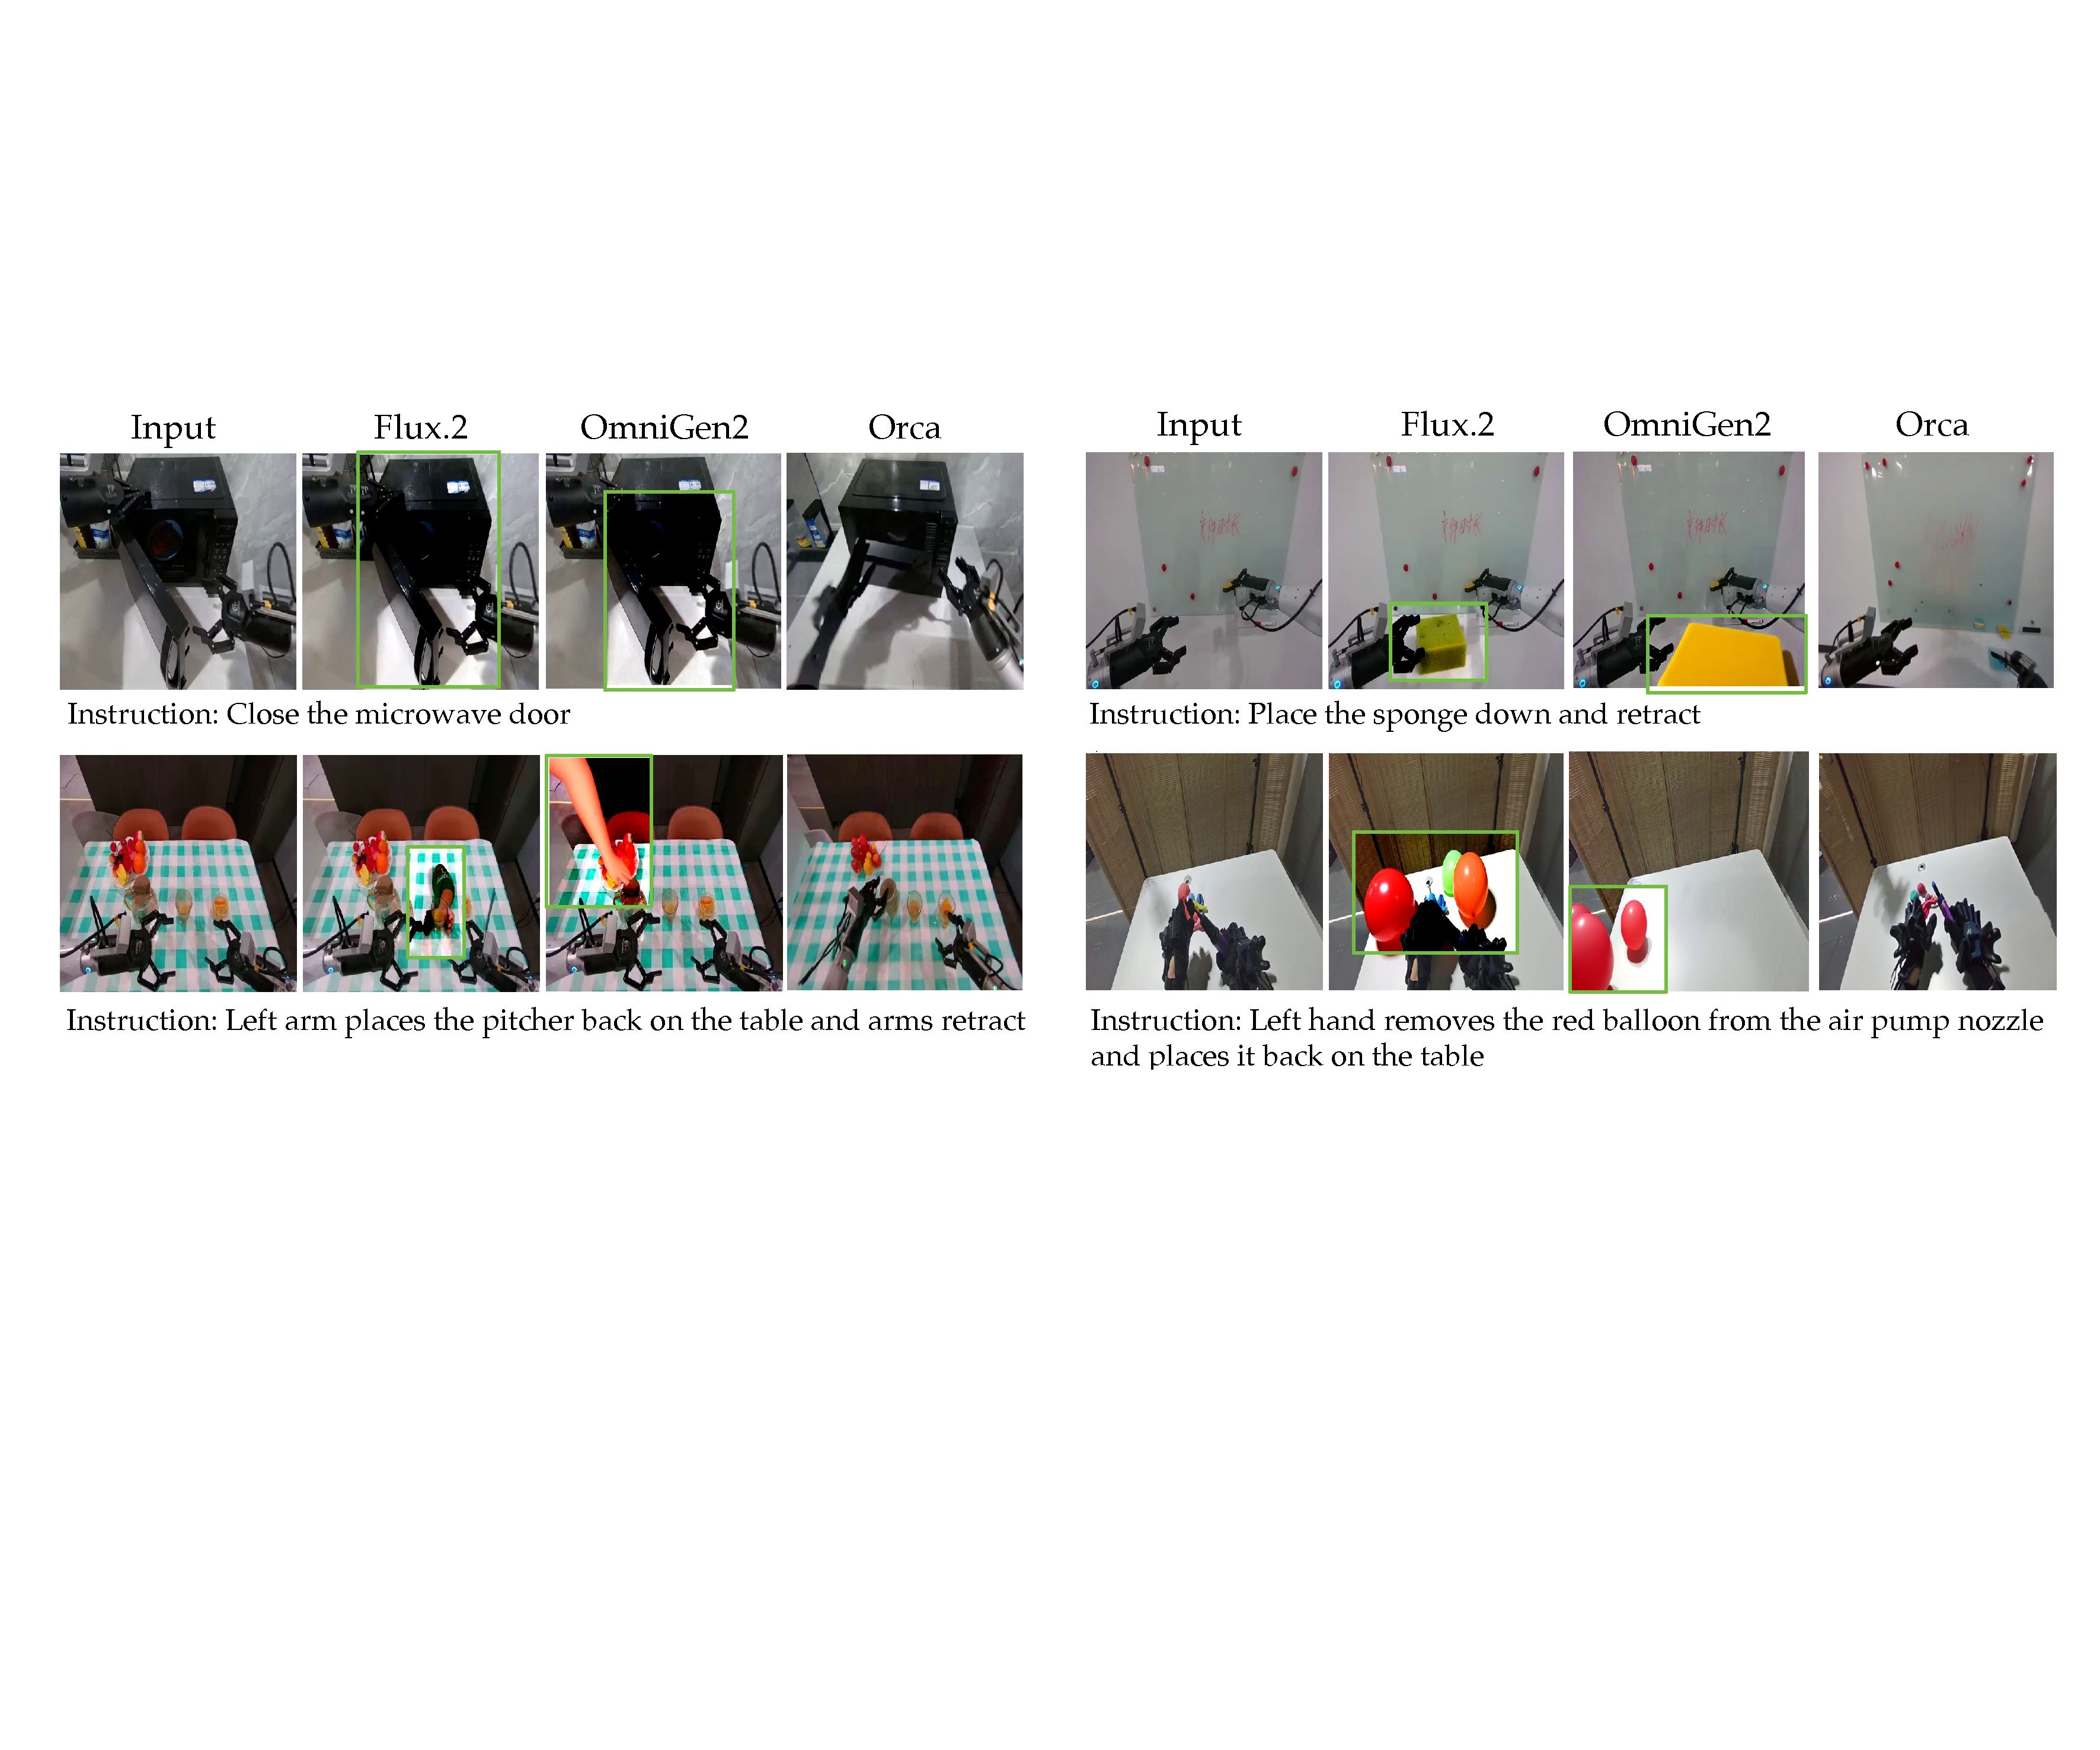
\includegraphics[width=1\linewidth]{figs/evaluation/ToV_visualization.pdf} 
    \caption{\textbf{Visual comparison of image prediction in the real world.}}
    \label{fig:tov_qualitative_main}
    \vspace{-0.3em}
\end{figure}



\begin{enumerate}[
    leftmargin=1.35em,
    itemsep=0.35em,
    topsep=0.35em,
    parsep=0em
]
    \item[] \textit{\textbf{1) Orca's learned world latent transfers effectively to image readout.}} 
    Compared with recent image generation baselines, Orca achieves the best average performance on PRICE and remains competitive across different real-world interaction sources. 
    This indicates that the learned world latent contains predictive information about future visual states under real-world interactions.

    \item[] \textit{\textbf{2) Orca better predicts interaction-conditioned state changes.}} 
    As shown in Figure~\ref{fig:tov_qualitative_main}, general image generation baselines suffer from typical flaws, such as the appearance or teleportation of irrelevant objects, hallucinatory human hands, poor instruction adherence, and biases stemming from prior knowledge. Orca better preserves robot morphology, scene and object consistency, contact relationships, and instruction following.
\end{enumerate}

These results suggest that the learned world latent provides useful state-transition information for visual readout, enabling more physically grounded image prediction for real-world interactions.


\subsubsection{Comparison on Action Generation}\label{sec:evaluation_toA}
To truly apply state transition modeling capabilities to the real world, we performed the embodied real-robot tasks. The details of benchmarks, metrics, and baselines are shown in \textbf{Appendix \ref{sec:appendix_evaluation_toA}}.

\paragraph{Benchmarks.} 

We used a dual-arm wheeled robot to collect data on five tasks: \textit{Take Book}, \textit{Stacked Bowls}, \textit{Pull Out Tissue}, \textit{Stamp}, and \textit{Scoop Sugar}. We performed two OOD settings: \textit{environment} and \textit{object OOD}. 

\paragraph{Metrics.} 
We report the rule-based scores, which measure key-stage task completion. The rule-based score is shown in Table \ref{tab:real_robot_scoring}.
We further employ PRM-as-a-Judge series~\citep{PRM-as-a-Judge, judge1.5} to provide dense trajectory-level diagnostics.


\paragraph{Baselines.} 
We compare Orca with V-JEPA 2.1~\citep{V-JEPA-2.1}, Qwen3.5~\citep{qwen35}, and $\pi_{0.5}$~\citep{pi0.5}. 
For V-JEPA 2.1 and Qwen3.5, we connect them to the same \textit{Action Expert} as Orca, i.e., V-JEPA 2.1 w/ AE and Qwen3.5 w/ AE, so that the comparison reflects the quality of the learned latent for action readout. V-JEPA 2.1 uses the latent as conditions, and Qwen3.5 uses the last hidden state as conditions. The remaining inputs of \textit{Action Expert} and training steps are consistent with Orca.
We also compare with $\pi_{0.5}$ as a strong VLA baseline pre-trained on large-scale robot data. 



\begin{table}[t]
  \centering
  \small
  \setlength{\tabcolsep}{2.7mm}
  \begin{threeparttable}
  \caption{\textbf{Comparison on action generation.} $\uparrow$ represents the higher value, the better, and vice versa.
  The metrics are trajectory-level diagnostics from PRM-as-a-Judge. \textbf{Note} that the backbones of all methods are frozen, and \textit{Action Experts} for Orca, V-JEPA 2.1, and Qwen3.5 are trainable from scratch.}\label{tab:comparison_changing_world}
    \begin{tabular}{c|c|cccccccc}
    \toprule[1pt]
    \textbf{\textit{Environment OOD}}& Rule-based $\uparrow$ & M25 $\uparrow$\tnote{1} & M50 $\uparrow$\tnote{1} & SR $\uparrow$\tnote{2} & MaxP-F $\uparrow$\tnote{3} &  FNS $\uparrow$\tnote{4} & DRR $\uparrow$\tnote{5}  & SQS $\uparrow$\tnote{6} \\
    \midrule[0.5pt]
    V-JEPA 2.1 &15.2  & 40    & 12    & 0     & 23.0   & 13.9   & 25.8  &  0.0\\
    Qwen3.5 & 12.4  & 26    & 10    & 0     & 18.3   & 11.2   & 19.2  &  0.0\\
    $\pi_{0.5}$ & 27.6  & 54    & \textbf{16} & 2     & 27.9  & 17.7   & 31.5  &  1.5\\
    \rowcolor[rgb]{ .89,  .949,  .851}\textbf{Orca} &\textbf{36.6} & \textbf{64} & \textbf{16} & \textbf{4} & \textbf{33.9}   & \textbf{19.3}  & \textbf{32.9} & \textbf{1.8} \\
    \midrule[1pt]
    
    \multicolumn{1}{c}{\textbf{\textit{Object OOD}}} & Rule-based $\uparrow$   & M25 $\uparrow$ & M50 $\uparrow$ & SR $\uparrow$ & MaxP-F $\uparrow$ & FNS $\uparrow$  & DRR $\uparrow$  & SQS $\uparrow$ \\
    \midrule[0.5pt]
    V-JEPA 2.1 &18.8  & 14    & 2     & 0     & 11.8  & 6.3    & 15.2  & 0.0 \\
    Qwen3.5 & 8.6   & 10    & 0     & 0     & 7.9   & 4.0     & 4.61  & 0.0\\
    $\pi_{0.5}$& \textbf{31.2} & \textbf{54}    & \textbf{12} & \textbf{8} & \textbf{25.1}  & \textbf{12.9}   & 21.9  & \textbf{4.5} \\
    \rowcolor[rgb]{ .89,  .949,  .851}\textbf{Orca} & 28.2  & 46 & \textbf{12}    & \textbf{8} & 21.8  &  10.8 & \textbf{27.7} & 3.9 \\
    \midrule[1pt]
    
    \multicolumn{1}{c}{\textbf{\textit{Overall}}} &  Rule-based $\uparrow$   & M25 $\uparrow$ & M50 $\uparrow$ & SR $\uparrow$ & MaxP-F $\uparrow$ & FNS $\uparrow$ & DRR $\uparrow$  & SQS $\uparrow$ \\
    \midrule[0.5pt]
    V-JEPA 2.1 & 17.0  & 27    & 7     & 0     & 17.4  & 10.1    & 20.5  & 0.0 \\
    Qwen3.5 & 10.5  & 18    & 5     & 0     & 13.1  & 7.6     & 11.9  & 0.0 \\
    $\pi_{0.5}$  & 29.4  & 54    & \textbf{14} & 5     & 26.5  & \textbf{15.3}   & 26.7  & \textbf{3.0} \\
    \rowcolor[rgb]{ .89,  .949,  .851}\textbf{Orca} & \textbf{32.4} & \textbf{55} & \textbf{14}    & \textbf{6} & \textbf{27.9} & 15.1 & \textbf{30.3} & 2.9 \\
    \bottomrule[1pt]
    \end{tabular}%
    \begin{tablenotes}
        \footnotesize
        \item[1] M25 and M50 are Milestone25\% and Milestone50\%. They are the proportions of the trajectory reaching 25\% and 50\%.
        \item[2] SR is the binary Success Rate. The unit is \%.
        \item[3] MaxP-F is MaxProcess in Failure. It represents the max-level execution process in the failure.
        \item[4] FNS is Failure Near-Success Score. It measures the progress achieved by failed trajectories before termination.
        \item[5] DRR is the Drawdown Recovery Ratio. It measures recovery after the largest progress drawdown.
        \item[6] SQS is the Success Quality Score. It measures the stability, smoothness, and high quality in the success process.
    \end{tablenotes}
  \end{threeparttable}
\end{table}%


\paragraph{Results and Analysis.} 
Based on Table~\ref{tab:comparison_changing_world}, we obtained two conclusions:



\begin{enumerate}[
    leftmargin=1.35em,
    itemsep=0.35em,
    topsep=0.35em,
    parsep=0em
]
    \item[] \textit{\textbf{1) Orca's learning paradigm and learned world latent transfers effectively to action readout.}} 
    Under the from-scratch Action Expert, 
    Orca outperforms Qwen3.5 in all OOD settings, achieving a breakthrough from 0\% success rate. It is also comparable to the powerful pre-trained $\pi_{0.5}$. This indicates that Orca's learning paradigm has a significant effect on action generation.

    \item[] \textit{\textbf{2) \textbf{Orca consistently advances the task and recovers better from execution errors.}}} The metrics show that Orca is more likely to make meaningful intermediate progress during execution, while suffering less from stagnation. Its higher FNS indicates that even when a trajectory eventually fails, Orca can reach later task stages before termination. Its higher DRR suggests that Orca is better at correcting deviations and continuing the task after progress drops. Figure~\ref{fig:recovery_after_failure} provides a qualitative case.
\end{enumerate}

\begin{figure}[!htbp]
    \centering
    
\includegraphics[width=1\linewidth]{figs/evaluation/main.pdf}
\caption{
\textbf{Recovery after repeated grasp failures.}
Orca recovers from early spoon-grasp failures and eventually makes progress, while $\pi_{0.5}$ remains unstable with repeated failed attempts.
}
\label{fig:recovery_after_failure}
\end{figure}

These results suggest that Orca produces action trajectories that move further, get stuck less often, and recover more effectively after mistakes.

\vspace{-1em}
\subsection{Ablation}\label{sec:exploration}

In the current learning paradigm, there are three losses, i.e., \textit{1) Observation-only state transition} $\lambda_{\mathrm{obs}}$; \textit{2) Event-conditioned state transition} $\lambda_{\mathrm{evt}}$; \textit{3) VQA response generation} $\lambda_{\mathrm{vqa}}$. So we ablated the different losses. The ablation results are shown in Table \ref{tab:ablation}. The results in Table \ref{tab:ablation} demonstrate that:

\begin{table}[!htbp]
  \centering 
\caption{\textbf{Ablation results.} ``-'' means the setting does not work. The first three rows average two metrics, while the last two average all three. Text, image, and action denote the average scores on text benchmarks, PRICE-V0.1, and overall rule-based action evaluation.}\label{tab:ablation}%
    \begin{tabular}{ccc|ccc|c}
    \toprule[1pt]
     $\lambda_{\mathrm{obs}}$   & $\lambda_{\mathrm{evt}}$ & $\lambda_{\mathrm{vqa}}$ & Text Generation & 
     Image Prediction& Action Generation & \textbf{Average} \\
     \midrule[0.5pt]
     &    & \ding{51}  & 48.4 & - & 10.2 & 29.3 \\
     
     \ding{51}    & \ding{51}  &  &    -  & 58.2  & 30.9  & 44.6 \\
    \ding{51}&     &   \ding{51}  & 50.5 & - & \textbf{32.6} & 41.6 \\
    \midrule[0.5pt]
    &  \ding{51}  & \ding{51}    & 50.1 & 54.7 & 23.0 & 42.6 \\
    \rowcolor[rgb]{ .89,  .949,  .851}\ding{51}& \ding{51}    & \ding{51}    & \textbf{51.8} & \textbf{59.8} & 32.4& \textbf{48.0} \\
    \bottomrule[1pt]
    \end{tabular}%
    \vspace{-1em}
\end{table}%

\begin{enumerate}[
    leftmargin=1.35em,
    itemsep=0.35em,
    topsep=0.35em,
    parsep=0em
]
\item[] \textit{\textbf{1) The three pre-training objectives provide the most balanced downstream readouts.}}
When $\lambda_{\mathrm{obs}}$, $\lambda_{\mathrm{evt}}$, and $\lambda_{\mathrm{vqa}}$ are jointly used, Orca achieves the most balanced performance across text, image, and action readouts. This shows that the three objectives jointly constrain the world latent space from natural dynamics, semantic conditions, and language supervision.

\item[] \textit{\textbf{2) Observation-only transition is especially important for action readout.}} 
Adding $\lambda_{\mathrm{obs}}$ clearly improves action generation. This suggests that dense natural dynamics from continuous videos provide useful information about temporal changes, object motion, and local physical interactions, which are critical for real-robot action generation.

\item[] \textit{\textbf{3) Event-conditioned transition is the key supervision for vision readout.}} 
Image prediction requires the model to infer a target state under a semantic condition. $\lambda_{\mathrm{evt}}$ aligns language-described events with visual state transition, enabling Orca to predict instruction- or event-guided target states rather than only modeling unconditional visual dynamics.

\item[] \textit{\textbf{4) VQA response generation preserves the language interface and strengthens semantic grounding.}} 
$\lambda_{\mathrm{vqa}}$ enables Orca to maintain natural-language readout ability and provides semantic and commonsense constraints for the learned world latent space. When combined with the two state-transition objectives, it further improves the overall balance among different downstream readouts.
\end{enumerate}
